% ============================================================================
% Paper D — REDEM-SSM
%   A State-Space Architecture with Native Online Learning,
%   Meta-Adaptation, and Structural Plasticity
% ============================================================================
% Target: Neurocomputing (Elsevier), elsarticle.
% Compile: pdflatex PAPER_D.tex (run twice for cross-refs).
% Figures resolve via ../figures/ (extension-less basenames).
% ============================================================================
\documentclass[preprint,12pt]{elsarticle}

\usepackage{amsmath,amssymb}
\usepackage{booktabs}
\usepackage{graphicx}
\usepackage{url}
% elsarticle's default Computer Modern is a bitmap font set, on which
% microtype's font expansion is unavailable, so lmodern (scalable Type 1)
% is loaded first; this also removes the two Overfull hboxes that the
% plain elsarticle preamble produced.
\usepackage{lmodern}
\usepackage{microtype}
% one Related-work paragraph still overflows by ~6pt after protrusion and
% expansion; the extra stretch is only taken up by lines that cannot be
% broken acceptably, so no other paragraph is re-flowed.
\setlength{\emergencystretch}{1em}

\graphicspath{{../figures/}}

\newcounter{proposition}[section]
\renewcommand{\theproposition}{\arabic{section}.\arabic{proposition}}
\newenvironment{proposition}[1][]{%
  \refstepcounter{proposition}%
  \par\noindent\textbf{Proposition \theproposition} (#1)\ \itshape\ignorespaces
}{\par}
\newenvironment{proof}{\noindent\itshape Proof.}{\hfill$\square$\par\medskip}

\journal{Neurocomputing}

\begin{document}

\begin{frontmatter}

\title{REDEM-SSM: A State-Space Architecture with Native Online
Learning, Meta-Adaptation, and Structural Plasticity}

\author[a]{Yaming Hu\corref{cor1}}
\cortext[cor1]{Corresponding author. ORCID: 0009-0003-1406-0485.}
\ead{64687555@qq.com}
\address[a]{Independent Researcher, Guiyang, Guizhou, China}

\begin{abstract}
State-space models (SSMs) are a natural host for online learning under
domain shift, but it is unclear which adaptation mechanisms must be
native to the host rather than retrofitted. We instantiate four
REDEM mechanisms --- an online readout (M1), a slow-trace statistical
memory (M3), soft routing over trained specialist readouts (M4, this
host's instantiation of the framework's structural-plasticity slot),
and a state-norm homeostat (M5, this host's instantiation of the
stability-regulation slot) --- on a diagonal linear recurrence with a
log-uniform timescale
spectrum, following a falsifying 10-seed paired development sequence.
Three host requirements emerge. (i)~A linear readout cannot recover
the current token from a linearly-decayed state mixture (a
deconvolution impossibility for affine-linear exact recovery); the
readout must consume the additive
input path, which beats a Transformer+LoRA reference on every seed,
and fixed multiplicative gates do not substitute for learned
selectivity. (ii)~The state's role is statistical metadata: a
fast-channel exponential moving average tracks domain switches and
soft routing retains per-domain specialists. Under the clipped-linear
perplexity of this squared-loss RLS readout family, several stream
comparisons are floor-sensitive and reverse once clipped tokens are
excluded; forgetting gains and the state-norm-homeostat negative
result are robust. A
companion study shows the artifact belongs to the training objective,
not the output range: post-hoc simplex projection removes negative
mass without repairing stream scores, whereas a trained probabilistic
readout does. (iii)~A
state-norm homeostat restores full-state statistics on a two-domain
task but degrades on a four-domain benchmark and is excluded from the
full stack. On that benchmark the full stack beats the bare host and
the untuned Transformer+LoRA reference on every seed on forgetting
(stream margins against the bare host are floor-sensitive). All
results are CPU-scale proofs of concept; we make no scaling claims.
\end{abstract}

\begin{keyword}
online learning \sep
state-space models \sep
continual learning \sep
reservoir computing \sep
homeostatic regulation \sep
timescale coverage
\end{keyword}

\end{frontmatter}

\section{Introduction}
\label{sec:intro}

Online sequence models must adapt while the stream is still running:
domain switches, non-stationary statistics, and long-horizon context
arrive without an offline retrain. State-space models (SSMs) replace
the frozen feedforward stack of Transformers with a recurrence whose
timescales can be designed rather than only learned
\cite{gu2022s4,gu2023mamba}, and they inherit a structural kinship
with reservoir computing: a fixed substrate, a trainable readout, and
an explicit separation between dynamics and plasticity
\cite{lukosevicius2009,jaeger2001esn}. The open design question is
\emph{which} adaptation mechanisms must live natively in such a host.

The REDEM framework couples four such mechanisms: a continuously
updated online readout (M1), a slow exponential trace --- an
exponential moving average (EMA) of the fast channels --- that
supplies statistical memory (M3), structural plasticity (M4), and a
homeostatic regulator that keeps the substrate at a stable operating
point (M5) --- the substrate-level regulation of the adaptation
process itself is the framework's \emph{meta-adaptation}
\cite{redemb}. A numbering note before we use these labels: the
companion papers number mechanisms per \emph{function} (in B, M4 is
coupling-graph rewiring and M5 a chaos homeostat), whereas this paper
numbers per \emph{host slot} and instantiates them differently --- here
M4 is soft routing over trained specialist readouts (a host-specific
instantiation of the gradual-structural-change design principle of
\cite{redemc}, not graph rewiring) and M5 a state-norm homeostat on
the whitened-state statistics. We use the companion numbering
throughout (M1, M3--M5) with that instantiation convention stated
once here; M2, the reward-gated plasticity mechanism of \cite{redemb},
is not
required by the RLS-only readout constraint adopted here and is not
instantiated on this host. A companion study \cite{redemc} tested the
same mechanism set on a Transformer host with low-rank adapters:
slow-trace domain
routing transferred (forgetting $-28\%$, 10/10 seeds) while a
gating-only variant was falsified at every tested metadata timescale
(0/10). That work explicitly did \emph{not} test a frozen-feedforward
host and did \emph{not} claim a general host boundary; the constructive
reading it supports --- a persistent stateful host rather than a
retrofit onto a static architecture, for the state-carrying mechanisms
that transferred there --- is the reading this paper takes as a design
premise and tests by building the host.

This paper takes the constructive consequence. We design a stateful
host --- a diagonal linear state-space recurrence with a log-uniform
timescale spectrum (the timescale-coverage principle of
\cite{redemc}) --- and instantiate M1, M3, M4, and M5 natively.
Rather than asserting that the design works, we follow the falsifying
discipline of the companion work: every claim is a paired 10-seed
comparison with sign consistency, and the negative results are
reported as design evidence, not as failures.

The development sequence produced three host requirements that are
the paper's main contribution:

\begin{enumerate}
\item \textbf{The readout needs a calibrated input path, not a
   clipped state mixture}
   (Section~\ref{sec:p1}). Exact recovery of the current token from a
   linearly-decayed state mixture is a deconvolution impossibility
   (Proposition~\ref{prop:p1}). Under the clipped-linear stream metric,
   every state-feature arm fails out of sample (0/10 vs.\ the
   Transformer+LoRA reference); that ranking is a \emph{calibration}
   property, not an absence of linear information --- coverage-spectrum
   state arms achieve lower unclipped CE while parking $10$--$12\%$ of
   tokens on the clip floor (the log-normal arms park $7.5$--$8.3\%$),
   whereas the input path produces
   non-positive scores on only $\sim$1.6\% of tokens. Fixed Mamba-style
   gates do not repair calibration (both $\gamma\in\{1,5\}$); selectivity
   must be learned (a boundary we flag, not cross).
\item \textbf{The state's role is statistical metadata}
   (Section~\ref{sec:p2}). A fast-channel state EMA (M3) tracks domain
   switches and routing over domain specialists (A3) retains them:
   forgetting improves at $\tau_m\le1000$ under both the reported and
   the unclipped metric. The pause-learning policy (A2) does \emph{not}
   pass the paper's own rubric: its reported stream gain over A1
   reverses once A1's clip floor is removed, and forgetting is never
   better than A1 at $\tau_m\in\{200,500\}$ and is only weakly better
   at larger $\tau_m$.
\item \textbf{Specialist retention beats a single stream readout, and
   state regulation is conditional}
   (Section~\ref{sec:p3}). At the tested $\tau_m{=}500$ point, soft
   routing retains purer forgetting than a bare single readout, while
   abrupt hard switching retains purer specialists than soft routing
   on forgetting; the reported soft-over-abrupt \emph{stream} margin
   reverses under the unclipped metric (Section~\ref{sec:sens}). A
   state-norm homeostat (M5) bounds the state and restores the
   full-state EMA as a valid domain statistic \emph{on the two-domain
   task only}. On the four-domain benchmark M5 degrades both metrics
   and is excluded from the full stack (Section~\ref{sec:p4}).
\end{enumerate}

None of the constituent mechanisms is individually new --- input-path
features, softmax routing, fast-channel EMAs, and norm feedback are
known primitives --- so the contribution claimed here is the
falsifying development sequence itself, the demonstration of which
mechanism combination a stateful host needs natively, and the
log-uniform timescale spectrum as the host-design choice. This is a
host-design study in the reservoir/online-readout lineage
\cite{jaeger2001esn,jaeger2004science,maass2002lsm}, not a claim of a
new sequence architecture.

On a four-domain irregular-switch benchmark the full stack beats the
bare host and the Transformer+LoRA reference on every seed (the
reference untuned for four domains; tuned, its stream margin narrows
to $-1.68$ while its retention collapses, Section~\ref{sec:p4}), and
the result transfers to a two-book real-text protocol
(Section~\ref{sec:p4}). All experiments are CPU-only and tiny by
design (scaling disclaimed in Section~\ref{sec:lim}).

\section{Related work}
\label{sec:related}

\paragraph{State-space sequence models and online adaptation.}
State-space models replace the frozen feedforward stack of
\cite{vaswani2017} with a recurrence whose parameters are trained
end-to-end (\cite{gu2022s4,gu2023mamba,liu2025longhorn,behrouz2025titans});
online adaptation has been pursued by rewriting the state with a learned
optimizer (\cite{sun2024ttt}) and by linear-attention delta updates
(\cite{yang2024deltanet}). Those hosts train with backpropagation and
typically assume a large pretrained parameter set, whereas the REDEM
line (\cite{redema,redemb,redemc}) restricts the readout to an online,
local rule on a fixed substrate. Our host therefore sits closer to the
designable-timescale end of the SSM spectrum than to end-to-end
selective SSMs such as Mamba.

\paragraph{Reservoir computing and fixed-substrate readouts.}
The fixed-substrate, readout-only split is classical in reservoir
computing: echo-state networks and liquid state machines run a fixed,
randomly generated recurrent substrate and train only a linear readout
(\cite{jaeger2001esn,jaeger2004science,maass2002lsm,verstraeten2007},
surveyed in \cite{lukosevicius2009}). Our host shares that split, but
replaces the randomly wired reservoir with a diagonal linear
recurrence whose log-uniform timescale spectrum is the design degree
of freedom that the readout and the metadata consume; nothing
recurrent is trained, and the adaptivity lives entirely in the online
readout and the routing mechanisms
(Sections~\ref{sec:m1}--\ref{sec:m4}). Relative to classical ESNs, the
paper's contribution is not a new reservoir topology but a controlled
account of which auxiliary mechanisms (input-path features, metadata
EMAs, soft specialist routing, optional homeostat) the host needs
under non-stationary streams.

\paragraph{Continual and online learning practice.}
Continual-learning practice emphasizes stability--plasticity trade-offs
and non-stationary evaluation (\cite{parisi2019}); online convex
optimization supplies the regret-theoretic frame for linear predictors
updated per round (\cite{zinkevich2003,cesabianchi2006}). Our
evaluation protocol follows that spirit --- paired per-seed stream and
forgetting perplexity under known and irregular domain switches ---
but the scientific object is the \emph{host requirement}, not a new
regularizer or a new continual-learning algorithm class. Our
Transformer+LoRA reference (\cite{hu2022lora}, retrained per task as
in \cite{redemc}) is a tiny parameter-efficient adapter and is not
compared against larger models (Section~\ref{sec:lim}); a classical
reservoir+RLS baseline is architecturally close to our bare host, so
we additionally run a separately wired ESN+RLS control on the identical
protocol and metrics (Section~\ref{sec:esn}); it fails out of sample.

\section{Methods}
\label{sec:methods}

\subsection{Host: diagonal state-space recurrence}
\label{sec:host}

The host is a diagonal linear recurrence
\begin{equation}
h_t = A\, h_{t-1} + B e_{t-1}, \qquad
A = \operatorname{diag}\big(e^{-1/\tau_i}\big),
\label{eq:recur}
\end{equation}
where $e_{t-1}$ is the one-hot token at step $t-1$, $B \in
\mathbb{R}^{N \times V}$ is a fixed random input projection
(entries drawn i.i.d.\ $\mathcal{N}(0, 1/N)$, per-seed), and the
timescales $\tau_i$ are drawn log-uniformly over $[1, 3000]$ tokens
($N = 128$, $V = 32$). The log-uniform spectrum realizes the
timescale-coverage principle of \cite{redemc}: fast channels carry the
recent token, slow channels carry long-horizon statistics. The state is
spectrum-whitened,
\begin{equation}
h^w_t = h_t \odot \sqrt{N\,(1 - A^2)},
\label{eq:whiten}
\end{equation}
which normalizes each channel to stationary unit variance (the
steady-state scaling of the linear recurrence) and bounds slow-channel
magnitude; without it the slow channels accumulate and the RLS
covariance grows as $(1/\lambda)^t$ in unexcited directions.

\subsection{M1: online RLS readout on the input path}
\label{sec:m1}

The readout is a per-token recursive-least-squares linear map
\begin{equation}
\hat{y}_t = W\, \phi_t, \qquad \phi_t = [\,B e_{t-1};\; 1\,],
\label{eq:readout}
\end{equation}
with $W \in \mathbb{R}^{V \times (N+1)}$ updated online (predict
before update) against the one-hot target $e_t$ with forgetting factor
$\lambda = 0.9999$ --- the classical recursive-least-squares family
(\cite{ljung1983,haykin2002,goodwin1984}), also an instance of online
convex optimization for linear predictors
(\cite{zinkevich2003,cesabianchi2006}) --- and with the inverse
covariance initialized as $P_0 = \delta I$ with $\delta = 1$. The cost
is $O(F^2)$ per token in the feature
dimension $F = N+1$, not $O(P^2)$ in a parameter count
\cite{redemb,redemc}. The squared-loss readout output is a linear
minimum-mean-square-error (MMSE)
estimate of the conditional distribution, so perplexity is evaluated as
the cross-entropy
$\mathrm{CE} = -\ln\,\mathrm{clip}(\hat{y}_t[e_t], 10^{-12}, 1)$
\emph{without} a softmax (a softmax double-normalizes the estimate
toward uniform).
The fraction of non-positive scores, $\mathrm{neg\_frac}$
($\hat y_t[e_t]\le 0$), is reported as a diagnostic. Because clipping
removes the standard probabilistic
meaning of perplexity, cross-arm comparisons inherit the clip range.
We therefore report, for every SSM arm, the clip fraction
$\mathrm{clip\_frac}$ (tokens with $\hat y_t[e_t]\le10^{-12}$, the
true floor hits of the CE definition above --- in all measured arms this
coincides with $\mathrm{neg\_frac}$, because scores in
$(0,10^{-12}]$ were never observed),
the holdout counterparts $\mathrm{forget\_neg\_frac}$ /
$\mathrm{forget\_clip\_frac}$, and two unclipped diagnostics ---
$\mathrm{ppl}_{\mathrm{unclipped}}$ (each arm on its own
$\hat y>0$ tokens) and a same-token-set rescore of every pair on the
intersection of their $\hat y>0$ supports (Section~\ref{sec:sens}).
Per-token arrays enabling the same-token-set rescore are written under
\texttt{data/per\_token/}. The
unclipped metrics are \emph{sensitivity analyses}, not a replacement
headline: selection bias remains for the per-arm form, the same-token
set still drops tokens on which either arm clips, and both are
undefined for arms with no
non-positive scores under this evaluation (the Transformer+LoRA
reference uses softmax cross-entropy and has no clip floor).
Section~\ref{sec:sens} tabulates which conclusions survive the floor
removal.

The input-path feature choice is itself an evidence-driven result
(Section~\ref{sec:p1}); the whitened state $h^w$ is \emph{not} a readout
feature.

\subsection{M3: fast-channel metadata EMA}
\label{sec:m3}

M3 is a per-token exponential moving average of the fast channels of the
whitened state,
\begin{equation}
m_t = \left(1 - \tfrac{1}{\tau_m}\right) m_{t-1} +
\tfrac{1}{\tau_m}\, h^w_t[\mathrm{fast}], \qquad \tau_i \le 8
\text{ tokens},
\label{eq:ema}
\end{equation}
with $\tau_m \in \{200,500,1000,2000\}$. The fast channels (which
converge in a few tokens) are a stationary domain statistic; the full
state is not --- its slow channels accumulate over the whole stream, so
an EMA of the full state drifts away from any fixed per-domain reference
and the detector never flips.
Fixed per-domain references are the mean fast-channel state over
1500-token reference streams generated per domain.

\subsection{M4: soft routing over trained specialists}
\label{sec:m4}

For $D$ domains, M4 maintains $D$ readouts $(W_d, P_d)$. Routing uses
continuous softmax weights over the EMA distances,
\begin{equation}
w_d = \frac{\exp(-\|m_t - r_d\|/\kappa)}{\sum_{d'}
\exp(-\|m_t - r_{d'}\|/\kappa)},
\qquad \kappa = 0.5 \times \text{median pairwise }\|r_d - r_{d'}\|,
\label{eq:soft}
\end{equation}
with the prediction $\hat{y}_t = \sum_d w_d\, W_d \phi_t$ and
$W_d, P_d$ updated with error scaled by $w_d$. Here $\kappa$ is the
soft-routing length scale (data-adaptive, of order the reference
separation), distinct from the substrate coupling strength $\kappa$ of the
companion substrate paper \cite{redema} (there $\kappa^{*}\in(25,30)$) and
from the E/I modulation ratio $\kappa$ of the silicon-nitride front-end;
the three are unrelated quantities. This instantiates the
gradual-structural-change design of \cite{redemc}; on this host the
reported soft-over-abrupt stream margin is floor-sensitive and is not
claimed as primary evidence (Section~\ref{sec:sens}).
Continuous softmax routing over specialist readouts is the online,
single-layer analogue of mixture-of-experts routing
\cite{shazeer2017moe}, and the gating-versus-gradual contrast echoes
the gating practice of recurrent networks \cite{hochreiter1997lstm}.
A second design detail, \emph{dormant-covariance refresh}, keeps the
inverse-covariance $P_d$ of every readout current with the feature stream
(weights frozen, $P$ updated with zero error). Section~\ref{sec:p3}
measures it in isolation: advancing the inverse covariances while the
readout weights stay frozen learns nothing, so the refresh is not what
carries the routing result.

\subsection{M5: state-norm homeostat}
\label{sec:m5}

M5 is a closed-loop controller on the whitened-state norm: the effective
time step is adjusted so that the norm is held in a band around its
target $\sqrt{N}$ (the whitening's unit-variance intent),
\begin{equation}
\Delta_t = \mathrm{clip}\big(\Delta_{t-1} + \eta\,(\|h^w_t\| - \sqrt{N}),
\; 1,\; \Delta_{\max}\big), \qquad
h_t = A^{\Delta_t} h_{t-1} + B e_{t-1},
\label{eq:m5}
\end{equation}
with $\eta = 0.05$, $\Delta_{\max} = 10$. M5 is a feedback regulator,
not a fixed normalization: it responds to the measured state and bounds
the slow-channel accumulation that otherwise makes the full-state EMA a
non-stationary statistic. M5 is evaluated as a mechanism on the
two-domain task (Section~\ref{sec:p3}) and is \emph{not} part of the
benchmark stack (Section~\ref{sec:p4}).

\subsection{Tasks and discipline}
\label{sec:tasks}

{\sloppy
\textbf{Two-domain protocol (s18)}: two biased-bigram Markov domains
(shift-1 / shift-7 with disjoint bias sets), alternating every 3000
tokens (known switch instants), 6 segments, 18k tokens. \textbf{Four-domain
benchmark}: four domains (shifts 1/3/7/11, disjoint 4-symbol
bias sets) on a cycling schedule with \emph{irregular} switch intervals
(Uniform 2500--3500), 8 segments, $\sim$24k tokens. All seed rules and
metrics (stream perplexity, forgetting perplexity on held-out previous
domain, post-switch adaptation time) follow \cite{redemc} verbatim.
Every comparison is paired per seed over 10 seeds with sign consistency
($n_{\mathrm{pos}}/10$); the Transformer+LoRA reference is the tiny
online-LoRA model of \cite{redemc} retrained on each task. Two
presentation conventions apply throughout: Figs.~\ref{fig:p1arms}
and~\ref{fig:bench} show per-arm means with $\pm1$ standard-deviation
error bars over the 10 seeds, Fig.~\ref{fig:routing} shows means only,
and per-seed paired differences are
summarized by sign consistency (and, where quoted, paired $t$ values)
rather than tabulated with confidence intervals --- the
sign-consistency counts, not the $t$ values, are the robustness
statistics, since extreme $t$ values are sensitive to single seeds.\par}

\section{Results}
\label{sec:results}

\subsection{P1/P3a: the readout needs the input path}
\label{sec:p1}

Fig.~\ref{fig:p1arms} shows stream perplexity on the two-domain protocol
(10 seeds) for the state-based readout arms and the input-path control,
against the Transformer+LoRA reference (TF-A1, 15.01; TF prefixes the
Transformer-host arms throughout). The stage labels P1--P4 --- and P3a,
the readout-arm sub-experiment --- are this paper's own development-stage
labels (set in the order the arms were built and falsified; the
companions use their own stage names and no shared label sequence is
implied). Every state-feature
readout --- log-normal spectrum (LN-raw 114.99, LN-whiten 115.87),
coverage spectrum (CV-whiten 81.31), with the current-token projection
added (CV-skip 58.47) --- is worse than the reference on every seed
(0/10) under the reported clipped-linear metric. The input-path control
($\phi = [B e_{t-1}; 1]$, no state)
reaches 11.75, better than the reference on 10/10 seeds ($-3.26$).
Proposition~\ref{prop:p1} shows why exact recovery is impossible; the
corollary below scopes the measured failure. The ranking under this
metric is a \emph{calibration} ranking (Section~\ref{sec:sens}):
coverage-spectrum arms park $10$--$12\%$ of tokens on the clip floor
and would look \emph{better} than the input path on unclipped CE, so
the design conclusion --- consume the additive input path --- is
stated as a requirement for calibrated next-token scores under the
squared-loss readout, not as a claim that the state lacks linear
information.

\begin{proposition}[Deconvolution impossibility for the linear state
readout]
Let the host be $h_t = \Lambda h_{t-1} + B e_{t-1}$ with
$\Lambda = \operatorname{diag}(\lambda_1,\dots,\lambda_N)$,
$0 < \lambda_i < 1$ distinct, and $B \in \mathbb{R}^{N\times V}$ with
i.i.d.\ continuous entries. For almost every such $(\Lambda, B)$, no
affine-linear readout $\hat e_t = U h_t + b$ recovers the most recent
input exactly ($\hat e_t = e_{t-1}$ for all token histories).
\label{prop:p1}
\end{proposition}
\noindent
Here $\Lambda$ is the host matrix $A$ of Eq.~(\ref{eq:recur}) with
entries $\lambda_i = e^{-1/\tau_i}$; we write $\Lambda$ inside the
proposition to avoid collision with the RLS forgetting factor $\lambda$
of Section~\ref{sec:m1}.

\begin{proof}
Unrolling the recurrence gives the mixture
$h_t = \sum_{j\ge0} \Lambda^j B e_{t-1-j}$ (with $e_{-1} = 0$). Exact
recovery for every history requires
$U B e_{t-1} = e_{t-1}$ for every token, i.e.\ $U B = I_V$, and
$U \Lambda^j B = 0$ for every $j \ge 1$. The annihilation conditions say
$U$ vanishes on $S = \operatorname{span}\{\Lambda^j B u : j \ge 1,\,
u \in \mathbb{R}^V\}$. Because the $\lambda_i$ are distinct and $B$ is
random, the Krylov family $\{\Lambda^j B\}_{j\ge0}$ generates
$\mathbb{R}^N$ almost surely (the $N$ vectors $\Lambda^{j} b_\ell$ for a
single random column $b_\ell$ form a Vandermonde system with distinct
nodes, hence are linearly independent a.s.), so
$S = \Lambda\,\operatorname{span}\{\Lambda^j B\}_{j\ge0} =
\Lambda\,\mathbb{R}^N = \mathbb{R}^N$ ($\Lambda$ is invertible). Hence
$U = 0$, contradicting $U B = I_V$. Whitening replaces $h_t$ by
$D h_t$ with a positive diagonal $D$ --- the elementwise whitening
scale of Eq.~(\ref{eq:whiten}), $\sqrt{N(1-\lambda_i^2)}$ per channel
--- i.e.\ $U' \mapsto U' D$; the
argument is unchanged, so the contamination is structural, not a scale
artifact.
\end{proof}

The empirical corollary of Proposition~\ref{prop:p1} is the measured
0/10 failure of every state-feature readout under the clipped-linear
stream metric: a pooled linear readout
cannot turn the state mixture into calibrated next-token scores, and
the input-path feature $\phi = [B e_{t-1}; 1]$ enters the state
equation as the $j{=}0$ term --- exactly the component the readout must
consume. Coverage-spectrum arms are not information-theoretically empty
(Section~\ref{sec:sens}): they achieve lower unclipped CE than the
input-path control while clipping far more often. The proposition
bounds \emph{exact} recovery; a boundary
analysis (data/s35\_readout\_boundary\_probe\_v1.csv) shows the
measured failure is a property of the pooled readout under this metric
rather than an absence of linear information. The probe is a linear
decoder fit by least squares on the first half of each stream (mapping
the whitened channels to the previous-token identity) and evaluated
out-of-sample on the second half by argmax agreement; chance is the
uniform 32-symbol vocabulary level ($1/32 \simeq 3.1\%$), and the
quoted ranges span per-channel, per-seed accuracies. The most recent
input token ($e_{t-1}$; called "the current token" at prediction time)
is
linearly decodable by argmax readout from the fast channels ($\tau_i \le 8$) of the
whitened state at 88.9--99.7\% out-of-sample accuracy (chance 3.1\%;
95.4--99.9\% with $\tau_i \le 30$), whereas the slow channels
($\tau_i \ge 100$) decode at chance (0.034--0.049): the older-token
contamination is a slow-channel property, and whitening rescales it
without removing it.

The in-sample ridge oracle is itself
window-dependent (28.8--33.4 on the full window vs.\ 16.2--18.4 on the
first half) and non-monotone in the feature set (adding the clean
projection makes it worse on every seed: 16.6--19.9 vs.\ 7.15--7.36 for
the projection alone) --- artifacts of evaluating clipped linear
outputs by perplexity, not bounds on recoverable information.
Restricting the readout to the fast channels does not repair the
next-token readout either: fast-channel-only linear fits and two-stage
decode-then-table compositions still fail out-of-sample (test ppl
68--104 vs.\ 13.9--17.4 for the pooled transition table fit on one half
and evaluated on the other) --- the token is linearly present, but the
closed-form squared-loss readout never turns it into calibrated
next-token probabilities, which is exactly what the input-path feature
achieves by encoding the token itself. Within
the RLS-only constraint the honest resolution remains the additive
input path.

Fixed Mamba-style multiplicative gates ($\hat{y} = W\,(h^w \odot
\sigma(\gamma C B e_{t-1}))$, $C$ fixed random, $\gamma \in \{1,5\}$)
do not repair the state readout: stream perplexity 77.19
($\gamma{=}1$) / 72.21 ($\gamma{=}5$); the sharper gate does not repair
it either (0/10 vs.\ the reference). Within the tested two-point
$\gamma \in \{1,5\}$ sampling the negative therefore does not appear to
be a tuning artifact; a wider gate-parameter grid was not swept, so we
state this design boundary only for the tested settings.
Selectivity in real Mamba-style hosts is
\emph{learned} end-to-end; a fixed random gate carries the previous
token only multiplicatively inside a time-varying state, which is noise,
not signal. Within our RLS-only constraint the honest resolution is the
additive input path --- which is what Mamba's input branch provides. We
flag the learned-selectivity route as the natural extension rather than
crossing the RLS-only boundary in this work.

\begin{figure}[t]
\centering
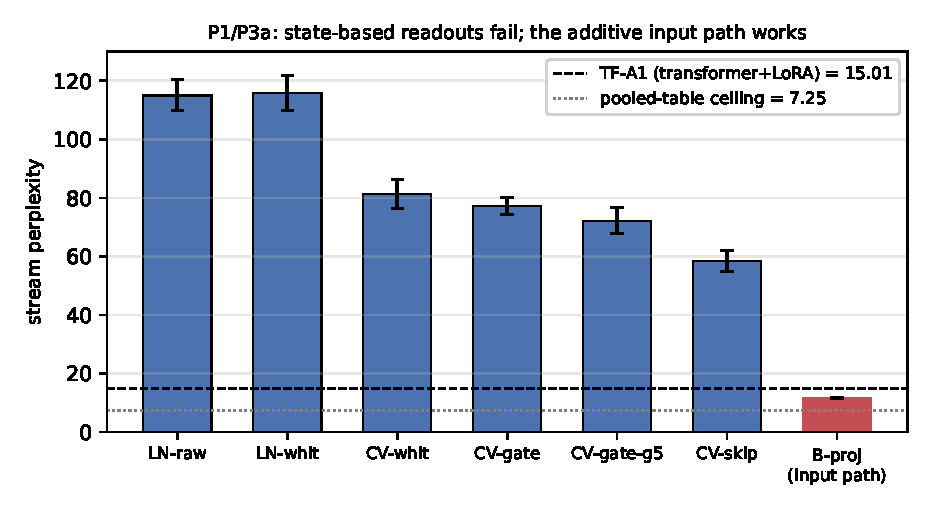
\includegraphics[width=0.9\linewidth]{paperD_fig1_p1_arms}
\caption{P1/P3a (10 seeds): stream perplexity of state-based readout arms
vs.\ the input-path control on the two-domain streaming task, under the
clipped-linear metric of Section~\ref{sec:m1}. All
state-feature readouts fail (0/10 vs.\ the Transformer+LoRA reference
TF-A1, dashed); fixed gates do not help; the additive input path
($B e_{t-1}$) reaches 11.75, below TF-A1, approaching the in-sample
pooled-table ceiling 7.25 (mean over seeds; range 7.15--7.36; the same
table fit on one half and evaluated on the other transfers at
$\sim$15 across the domain-mix shift, so the input path also beats the
non-adapting static table). The dotted line drawn inside the figure
marks this same 10-seed mean ceiling 7.25. This ranking is
floor-sensitive: see Section~\ref{sec:sens}.}
\label{fig:p1arms}
\end{figure}

\subsection{P2: routing transfers, gating is readout-dependent}
\label{sec:p2}

Table~\ref{tab:p2} and Fig.~\ref{fig:routing} (left). The three host
arms are A1 (bare: the input-path RLS readout only), A2 (the
pause-learning policy), and A3 (hysteresis-gated \emph{hard} routing
between two domain specialists --- a discrete nearest-reference
selector, not the soft weighting of M4, Eq.~\ref{eq:soft}). M3
(fast-channel EMA) supplies the domain statistic the
gate reads: over the 5 known switches of the two-domain protocol it
detects a mean of $2.80/5$ at $\tau_m{=}200$, falls to $0.30/5$ at 500,
and detects none at 1000 and 2000 (per-seed counts in
\texttt{switches\_detected}, data/s20\_ssm\_m3\_routing\_v1.csv) --- the
detector does not track the switching, yet the gate is still useful.
Routing (A3) with two domain specialists improves forgetting at
$\tau_m \le 1000$ under the reported metric ($-2.05$, $-1.87$, $-1.20$
ppl; 10/10 seeds) and is neutral at 2000 ($-0.01$, 5/10; the per-seed
paired-difference mean is $-0.007$, rounded to the table's two-decimal
convention in Table~\ref{tab:p2}). The 2000 neutrality is itself
floor-sensitive: under both unclipped scorings the $\tau_m{=}2000$
forgetting gain is robust ($-1.28$ per-arm unclipped / $-1.07$
same-token-set, 10/10; Section~\ref{sec:sens}) --- the clip floor
masks this gain rather than creating it.
The forgetting gain is largest where the detector
still fires: seeds with at least one detection gain $-1.99$ ppl on
forgetting against $-0.98$ for seeds with none. The detector is
therefore not what makes the routing work --- the gain survives at
$\tau_m{=}1000$, where it never fires --- but it marks where the gain is
strongest under the reported metric. A3's stream
cost in the frozen-covariance variant ($+0.38$ to $+4.08$) disappears in
the M4 variant that routes softly \emph{and} trains the specialists
online, which changes the routing rule and the specialist update
together (Section~\ref{sec:m4}, Section~\ref{sec:p3}).

The pause-learning arm (A2 --- the paused-readout policy, distinct from the
fixed multiplicative feature gates of Section~\ref{sec:p1})
appears to improve stream perplexity at every tested
$\tau_m$ under the reported clipped-linear metric ($-1.52$ to $-2.45$,
10/10), the opposite of the companion's A2 falsification (0/10). That
stream margin does not survive floor removal: A2 itself clips on only
$\sim4\times10^{-5}$ of stream tokens, while A1 clips on $1.58\%$, so
the reported A2-over-A1 gain is largely A1's floor penalty. Under the
unclipped metric A2 is \emph{worse} than A1 on stream at every
$\tau_m$ ($+1.45$ to $+2.38$, 0/10). Forgetting --- already printed in
Table~\ref{tab:p2} --- is worse than A1 at $\tau_m\in\{200,500\}$
($+0.52$, 0/10; $+0.03$, 5/10) and only weakly better at
$\tau_m\in\{1000,2000\}$ ($-0.23$, 10/10; $-0.37$, 9/10); under the
unclipped metric those large-$\tau_m$ gains shrink further
($-0.04$, 8/10; $-0.18$, 9/10). By the paper's own rubric ---
a pause policy must not buy stream by sacrificing retention --- A2
does not pass. Two honest comparisons with the companion remain: the
companion's A2 paused LoRA plasticity while keeping the head active,
whereas here pausing the only trainable component pauses all learning;
and the companion's 0/10 falsification used a fast Adam/LoRA readout
whose within-domain knowledge decays when paused, while this RLS
readout stays near the pooled-table optimum. The pause policy's effect
is therefore readout-dynamics-dependent \emph{and}, on this host,
metric-dependent. We report this qualification rather than editing the
companion paper.

\begin{table}[t]
\centering
\small
\begin{tabular}{lccccc}
\toprule
arm & $\tau_m$ & stream & $\Delta_{\mathrm{ppl}}$ & forget &
$\Delta_{\mathrm{forget}}$ \\
\midrule
A1 bare & --- & 11.75 & --- & 8.39 & --- \\
A2 pause & 200 & 10.24 & $-1.52$ (10/10) & 8.91 & $+0.52$ (0/10) \\
A2 pause & 500 & 9.53 & $-2.22$ (10/10) & 8.42 & $+0.03$ (5/10) \\
A2 pause & 1000 & 9.30 & $-2.45$ (10/10) & 8.15 & $-0.23$ (10/10) \\
A2 pause & 2000 & 9.70 & $-2.05$ (10/10) & 8.02 & $-0.37$ (9/10) \\
A3 route & 200 & 12.14 & $+0.38$ (0/10) & 6.33 & $-2.05$ (10/10) \\
A3 route & 500 & 13.30 & $+1.55$ (0/10) & 6.52 & $-1.87$ (10/10) \\
A3 route & 1000 & 14.81 & $+3.06$ (0/10) & 7.19 & $-1.20$ (10/10) \\
A3 route & 2000 & 15.83 & $+4.08$ (0/10) & 8.38 & $-0.01$ (5/10) \\
\bottomrule
\end{tabular}
\caption{P2 (10 seeds, two-domain protocol): routing (A3) retains domain
specialists (forgetting improves at $\tau_m \le 1000$, 10/10) at a
frozen-covariance stream cost that disappears in the M4 variant which
routes softly and trains the specialists online
(Section~\ref{sec:p3}). Pause-learning (A2 --- the paused-readout policy,
not the multiplicative feature gates of Section~\ref{sec:p1}) shows a
reported stream gain that reverses under the unclipped metric and a
forgetting cost at small $\tau_m$ (Section~\ref{sec:sens}).}
\label{tab:p2}
\end{table}

\subsection{P3: specialist retention at the tested point, and state
regulation is conditional}
\label{sec:p3}

Fig.~\ref{fig:routing} (right): at $\tau_m{=}500$, soft routing (M4,
Eq.~\ref{eq:soft}) improves forgetting over the bare single readout A1
($-1.99$ ppl, 10/10), while abrupt hard switching retains purer
specialists than soft routing on forgetting ($-2.37$ vs.\ $-1.99$ vs.\
A1; soft $-$ abrupt $=+0.38$ ppl, 1/10). Under the reported
clipped-linear metric soft also appears to beat abrupt on
\emph{stream} ($-1.81$ ppl, 10/10); that margin reverses under the
unclipped metric ($+0.76$, 0/10; Section~\ref{sec:sens}). We therefore
do not claim ``gentle wins'' on stream. Soft routing
with both specialists trained online improves the reported stream
result from the $+1.55$ of the hysteresis routing in
Table~\ref{tab:p2}, whose inactive readout is fully frozen, to $-3.54$
against the bare host (10/10) --- also floor-sensitive, since A1 clips
more than A3-soft ($1.58\%$ vs.\ $0.28\%$). Because
that comparison changes the routing rule and the training of the
specialists at once, we isolate the second factor
(data/s37\_dormant\_p\_probe\_v1.json): with the same soft routing but the
readout \emph{weights frozen} and only the inverse covariances refreshed,
stream and forgetting perplexity are both exactly 32.0 --- chance for the
32-symbol vocabulary --- on all 10 seeds, i.e. worse than the bare host by
$+20.2$ (0/10). Refreshing the covariance learns nothing; the entire gain
comes from training the specialists.

M5 (Eq.~\ref{eq:m5}) bounds the whitened-state norm (mean 11.3 in band
vs.\ 50.2 for the bare host, whose norm drifts upward on the slow
timescales --- a long transient toward a large but bounded steady state
under the switched, non-stationary stream, not unbounded growth; the
host is contractive), restores the \emph{full}-state
EMA as a valid domain statistic (5/5 switch detections vs.\ 0.6/5 ---
a switch counts as detected when the hysteresis nearest-reference
estimate on the metadata statistic flips to the incoming domain at the
known switch instant, and 0.6/5 averages the per-seed flip counts over
the bare host --- the
non-stationarity of Section~\ref{sec:m3} fixed at the source), and
recovers from a magnitude-10 state kick in $\sim$10 tokens
($\Delta_t$ settles near 5.4; the disturbance is a single-step
additive kick of magnitude 10 in a random unit direction applied to
the state at the first switch, and recovery is measured as the first
step at which the whitened-state norm returns to within the
$1.05\,\sqrt{N}$ band (the band's upper edge)). This is mechanism-level
evidence: on this
architecture the readout is decoupled from the state (input path), so a
direct ``stream performance under disturbance'' test is not meaningful
here. These two-domain results do not transfer to the four-domain
benchmark, where M5 is harmful (Section~\ref{sec:p4}).

\begin{figure}[t]
\centering
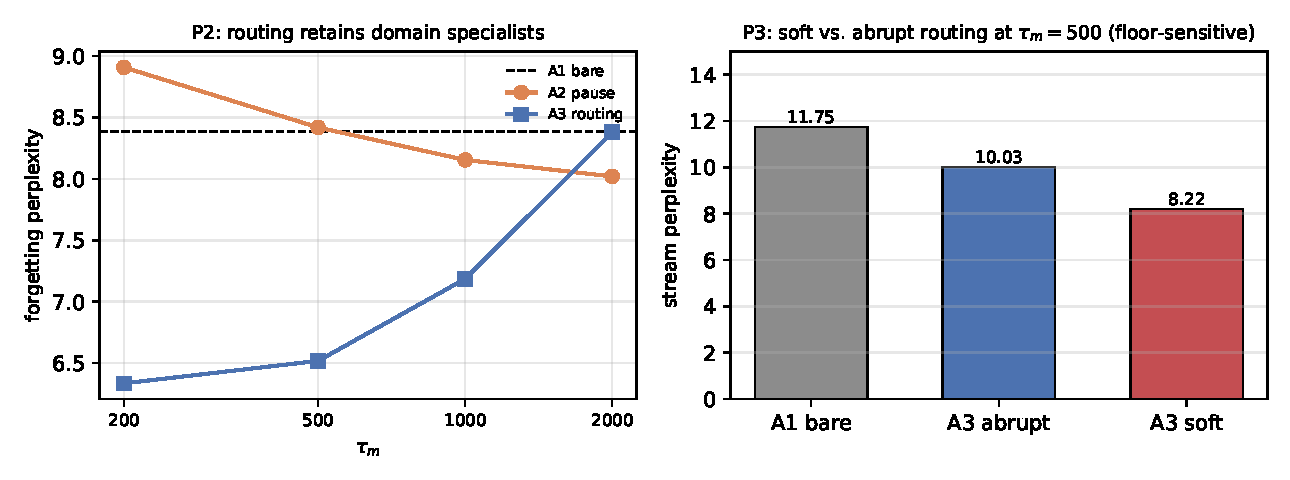
\includegraphics[width=0.9\linewidth]{paperD_fig2_routing}
\caption{Left (P2): forgetting perplexity vs.\ $\tau_m$ --- routing (A3)
retains domain specialists below the bare baseline (A1, dashed) at every
tested $\tau_m$; pause-learning (A2 --- the paused-readout policy of
Section~\ref{sec:p2}, not the multiplicative feature gates of
Section~\ref{sec:p1}) does not at $\tau_m \le 500$ and crosses below the
baseline only at the two slowest metadata timescales. Right (P3): soft
routing shows a lower reported stream perplexity than abrupt at the
tested $\tau_m{=}500$ point, but that margin reverses under the
unclipped metric (Section~\ref{sec:sens}); abrupt switching retains
purer specialists on forgetting.}
\label{fig:routing}
\end{figure}

\subsection{P4: benchmark on four-domain irregular switching}
\label{sec:p4}

{\sloppy
Fig.~\ref{fig:bench} and Table~\ref{tab:p4}. All P4 runs --- the
four-domain benchmark, the real-text transfer, and the follow-up
comparisons below --- use the $\tau_m{=}500$ selected by the P2 sweep
(with the data-adaptive $\kappa$ of Eq.~(\ref{eq:soft})), fixed
thereafter and not re-swept. The four-domain irregular-switch protocol
is a deliberate upgrade over the two-domain stage tasks (four domains,
irregular switch intervals, a longer stream of $\sim$24k vs 18k tokens): a more demanding
generalization test than the protocol on which the stage experiments
were run. On this protocol, the full stack (M1 input-path readout + M3
metadata + M4 soft routing) beats the bare host robustly on
\emph{forgetting} ($-4.47$ reported, $-4.53$ unclipped; 10/10 both).
The reported stream margin ($-2.25$, 10/10) reverses under the
unclipped metric ($+1.45$, 0/10) because SSM-bare clips on $1.16\%$ of
stream tokens while REDEM clips on $0.07\%$; we therefore treat the
P4 stream win as floor-sensitive and lead with retention. Against the
Transformer+LoRA reference the full stack wins on both axes under the
reported metric (stream $-9.28$, forgetting $-10.08$; 10/10); the
unclipped metric is undefined for TF-A1 (softmax CE, no clip floor).
Even the bare host beats the
transformer reference 10/10 on reported stream ($-7.03$): the RLS
readout's second-order convergence dominates online Adam
\cite{kingma2015adam}/LoRA when
domains switch faster than
the LoRA can track (the reference reaches only 22.46 ppl, below the
uniform-chance 32).\par}

\emph{Real-text transfer.} The same protocol on two public-domain books
(Alice's Adventures in Wonderland vs.\ A Tale of Two Cities, character
-level, case-folded, 32-symbol vocabulary) reproduces the result:
REDEM-SSM beats SSM-bare robustly on forgetting ($-0.46$ reported,
9/10; $-0.33$ unclipped, 9/10). The reported stream margin ($-1.26$,
10/10) nearly vanishes under the unclipped metric ($-0.05$, 7/10).
Against TF-A1 the full stack wins on both reported axes (stream
$-5.23$, forgetting $-2.01$; 10/10); even
the bare host beats TF-A1 10/10. The fast-channel metadata separates the
two sources, and soft routing retains per-source specialists, although
the forgetting gain is smaller than on the synthetic task --- the two
books share English letter bigram statistics, so their specialists
overlap more than the four synthetic domains'. The first-order readout
reaches the char-bigram regime (ppl $\sim$12--13); higher-order text
structure is out of its reach and is reported as a boundary, not a
result. A count-based bigram oracle pins this boundary quantitatively
(data/s31\_char\_bigram\_oracle\_v1.csv): the true per-source first-order
ceiling, estimated from the full books and evaluated on the same
per-seed windows, is ppl $10.97\pm0.18$ (stream) --- REDEM-SSM's 12.07
sits within $\sim$1.1 ppl of its structural ceiling (the residual is
finite-sample loss of the streaming readout), and the Transformer
reference (17.31) fails to reach even this first-order ceiling, so its
deficit is not about higher-order structure. One caveat on the
ceiling: it is fitted on the full books and evaluated on the same
per-seed windows, so it is in-sample for the evaluation window and
optimistic; a ref-window-fitted variant of the same oracle exists in
the released oracle data and is not quoted here, so the ``within
$\sim$1.1 ppl of ceiling'' statement should be read with that
convention in mind.

{\sloppy
\emph{Reference fairness and mechanism transfer (follow-up).} Two
legitimate objections to the TF-A1 comparison are that the reference
uses the untuned s18 hyperparameters and that it carries no routing
mechanism. We close both on the same four-domain protocol (10 seeds;
data/s26\_ssm\_p4\_fair\_tf\_v1.csv). (i) A small tuning grid (four
learning rates from $3\times10^{-4}$ to $10^{-2}$; ranks 16 and 32)
improves the bare reference's stream perplexity to 14.86 at
$\mathrm{lr}{=}3\times10^{-3}$, rank 32 --- still worse than REDEM-SSM
on 10/10 seeds ($-1.68$, paired $t=-8.8$; the best config's forgetting
collapses to 62.2
vs.\ 8.93, so the tuning that helps the stream destroys retention and
the default reference is the balanced representative). The P4 margin is
therefore robust to reasonable reference tuning, though smaller on
stream. (ii) The s18 routing mechanism (A3) generalized to four adapters
(TF-A3, $\tau_m{=}500$) recovers the specialists: forgetting drops from
19.01 to 10.84 ($-8.17$, 10/10) --- slow-trace routing transfers to the
Transformer host on this second protocol (Paper~C) --- but does not
repair the stream: TF-A3 stays at 21.77, losing to REDEM-SSM on 10/10
seeds ($+8.59$). The stream advantage of the input-path RLS readout is a
property of the stateful host, not of the routing mechanism: the
mechanisms transfer across the two hosts tested (with unequally tuned
reference baselines on the two hosts), and we do not claim
host-agnostic transfer beyond them --- the stream performance is not
host-agnostic.\par}

\emph{M5 in the benchmark (negative).} The P3 state-norm homeostat was
deliberately excluded from the P4 stack; adding it confirms the decision
empirically (data/s33\_ssm\_p4\_m5\_v1.csv): REDEM-SSM+M5 is \emph{worse}
on all 10 seeds (stream $+1.53$, forgetting $+2.90$; paired $t =
+22.8/+26.5$ on the same ordering). A plausible mechanism --- offered as an interpretation,
not a directly measured result --- is that the $\Delta_t$ modulation
departs from the per-channel whitening calibrated at $\Delta_t = 1$, so
the readout's features lose their calibrated scale on a stream that is
already well-conditioned (the norm never runs away --- mean $\Delta_t
\approx 5.3$ means the controller is constantly active). We have not
quantified the per-channel variance mismatch at $\Delta_t \approx
5.3$, nor run an M5-plus-recalibrated-whitening control, so this
attribution is a hypothesis; the empirical negative itself (all 10
seeds) is the solid part of the result. M5 remains a
mechanism-level safeguard for the spike regime (P3, E2), not a benchmark
component.

\begin{figure}[t]
\centering
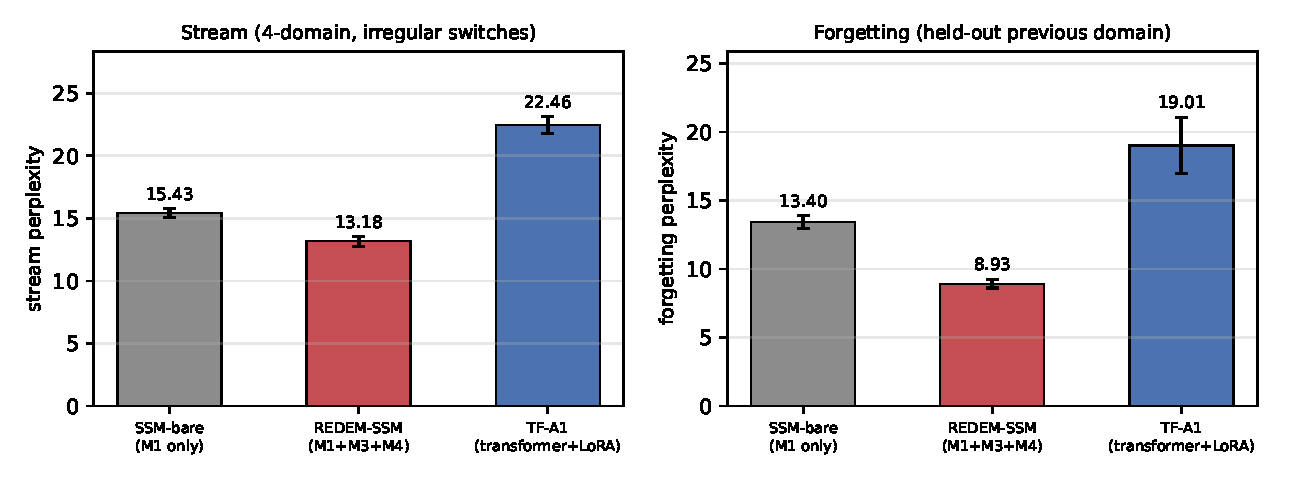
\includegraphics[width=0.9\linewidth]{paperD_fig3_benchmark}
\caption{P4 (10 seeds, four-domain irregular-switch protocol): the full
REDEM-SSM stack beats the bare host robustly on forgetting and the
Transformer+LoRA reference on both reported axes (paired, 10/10; stream
vs.\ bare is floor-sensitive, Section~\ref{sec:sens}).}
\label{fig:bench}
\end{figure}

\begin{table}[t]
\centering
\small
\begin{tabular}{lcc}
\toprule
arm & stream ppl & forgetting ppl \\
\midrule
SSM-bare (M1 only) & 15.43 & 13.40 \\
REDEM-SSM (M1+M3+M4) & \textbf{13.18} & \textbf{8.93} \\
\multicolumn{3}{l}{\scriptsize M4 = soft routing over specialist readouts;
M3 = fast-channel metadata (Introduction)} \\
TF-A1 (transformer+LoRA) & 22.46 & 19.01 \\
\midrule
\multicolumn{3}{l}{\scriptsize paired (10/10): REDEM--bare
$-2.25$/$-4.47$} \\
\multicolumn{3}{l}{\scriptsize stream floor-sensitive (unclipped
$+1.45$/$-4.53$); unclipped undefined for TF} \\
\multicolumn{3}{l}{\scriptsize REDEM--TF $-9.28$/$-10.08$;
bare--TF $-7.03$/$-5.61$} \\
\multicolumn{3}{l}{\scriptsize M3/M4 factor split and classical ESN
control: Tables~\ref{tab:m3m4}--\ref{tab:esn}} \\
\bottomrule
\end{tabular}
\caption{P4 (10 seeds, four-domain irregular-switch protocol): the full
stack (input-path RLS readout, fast-channel metadata, soft routing over
four specialists) beats the bare host robustly on forgetting and the
Transformer+LoRA reference on every seed under the reported metric.
The stream margin against the bare host is floor-sensitive
(Section~\ref{sec:sens}). The transformer reference uses the companion's
hyperparameters, untuned for four domains.}
\label{tab:p4}
\end{table}

\subsection{P4 factor ablation: what M3 and what M4 contribute}
\label{sec:m3m4}

Table~\ref{tab:p4}'s endpoints (M1 vs.\ M1+M3+M4, with M4 the soft-routing
instantiation of the Introduction's numbering note) do not separate the
benchmark roles of the fast-channel metadata (M3) and of soft routing
(M4). The factor ablation (data/s38\_ssm\_p4\_m3m4\_ablation\_v1.csv,
same seeds, protocol, and $\tau_m{=}500$ as Table~\ref{tab:p4}) adds two
intermediate arms: \emph{uniform}, four specialists trained with fixed
soft weights $1/4$ (M4 structure without M3 assignment), and
\emph{hard}, hard nearest-reference assignment on the M3 EMA with the
inactive specialist frozen (M3 assignment without soft mixtures).

\begin{table}[t]
\centering
\small
\begin{tabular}{lcc}
\toprule
arm & stream ppl & forgetting ppl \\
\midrule
SSM-bare (M1) & 15.43 & 13.40 \\
SSM-uniform (M4 without M3) & 15.89 & 12.98 \\
SSM-hard (M3 without soft M4) & 18.32 & \textbf{8.16} \\
SSM-REDEM (M1+M3+M4 soft) & \textbf{13.18} & 8.93 \\
\midrule
\multicolumn{3}{l}{\scriptsize uniform $-$ bare: $+0.46$/$-0.43$ (2/10, 9/10)} \\
\multicolumn{3}{l}{\scriptsize hard $-$ bare: $+2.90$/$-5.24$ (0/10, 10/10)} \\
\multicolumn{3}{l}{\scriptsize REDEM $-$ bare: $-2.25$/$-4.47$ (10/10, 10/10)} \\
\multicolumn{3}{l}{\scriptsize REDEM $-$ hard: $-5.14$/$+0.77$ (10/10, 2/10)} \\
\bottomrule
\end{tabular}
\caption{P4 M3/M4 factor ablation (10 seeds, same protocol as
Table~\ref{tab:p4}). Uniform specialists alone barely move either axis;
hard M3 assignment buys forgetting at a stream cost; soft M4 recovers
stream relative to hard routing while giving up a small forgetting
margin. Reported metric; unclipped values in the data file.}
\label{tab:m3m4}
\end{table}

Reading Table~\ref{tab:m3m4}: (i)~specialists without assignment
(uniform) are close to the bare host on stream ($+0.46$, 2/10) and only
weakly better on forgetting ($-0.43$, 9/10) --- M4 structure alone does
not carry the benchmark; (ii)~hard M3 assignment is what retains
specialists on forgetting ($-5.24$, 10/10) but pays on stream ($+2.90$,
0/10); (iii)~soft M4 recovers the stream margin relative to hard
routing ($-5.14$, 10/10) while remaining slightly worse than hard on
forgetting ($+0.77$; hard better on 8/10). The full stack therefore
works because M3 assignment provides domain memory and soft M4 turns
that memory into a stream-usable mixture --- not because either piece
alone is sufficient.

\subsection{Classical ESN+RLS baseline under the same protocol}
\label{sec:esn}

A separately wired random reservoir (ESN) with an online RLS readout on
the reservoir state is the classical fixed-substrate-plus-linear-readout
reference (Jaeger's echo-state network). We ran it on the identical P4
stream, seeds, and metrics (data/s40\_esn\_rls\_p4\_baseline\_v1.csv):
$r_t=(1-a)r_{t-1}+a\tanh(W_{\mathrm{in}}e_{t-1}+W_{\mathrm{res}}r_{t-1}+b)$
with sparse $W_{\mathrm{res}}$ scaled to spectral radius $\rho$, $a=0.5$,
input scaling $1$, and the same RLS recurrence as the SSM arms.

\begin{table}[t]
\centering
\small
\begin{tabular}{lcc}
\toprule
arm & stream ppl & forgetting ppl \\
\midrule
ESN-lin (one-hot control) & 12.43 & 13.41 \\
ESN-128 ($\rho=0.9$) & 98.78 & 97.76 \\
ESN-128 ($\rho=1.0$) & 99.69 & 95.30 \\
ESN-256 ($\rho=0.9$) & 97.10 & 87.83 \\
SSM-bare (Table~\ref{tab:p4}) & 15.43 & 13.40 \\
SSM-REDEM (Table~\ref{tab:p4}) & 13.18 & 8.93 \\
\bottomrule
\end{tabular}
\caption{Classical ESN+online-RLS on the P4 protocol (10 seeds).
Separately wired reservoirs fail out of sample on both axes (0/10 vs.\
the one-hot control and vs.\ SSM-bare/SSM-REDEM, seed-aligned).}
\label{tab:esn}
\end{table}

The classical ESN is far worse than the bare diagonal host with the
input-path readout (stream $98.8$ vs.\ $15.4$; paired
ESN-128 $-$ bare $=+83.4$, 0/10) and than the full stack
($+85.6$, 0/10). Wider reservoirs and edge-of-stability $\rho$ do not
close the gap. This is the same failure mode as the P1 state-mixture
readout: a linear readout on a decaying reservoir state mixture does not
calibrate next-token scores on this protocol. The bare M1 arm is not a
stand-in for a classical ESN --- the input path is a different topology
--- but a classical ESN does not rescue the host either. The one-hot
control (no reservoir, $12.4$) sits below the reported bare-host stream
($15.4$) only because that bare value is clip-inflated; on the unclipped
metric the bare host ($\approx 11.5$) is the better linear arm
(Section~\ref{sec:sens}).

\subsection{Metric sensitivity of the clipped-linear perplexity}
\label{sec:sens}

The squared-loss readout is scored by
$\mathrm{CE}=-\ln\,\mathrm{clip}(\hat y_t[e_t],10^{-12},1)$
(Section~\ref{sec:m1}). Each clipped token contributes a fixed
$-\ln(10^{-12})\simeq27.63$ nats. Table~\ref{tab:sens} compares every
headline paired difference under three scorings:
(i) the \emph{reported} clipped-linear metric;
(ii) the \emph{per-arm unclipped} sensitivity metric
($\mathrm{ppl}_{\mathrm{unclipped}}$, Section~\ref{sec:m1}; each arm
conditioned on its own $\hat y>0$ tokens);
(iii) the \emph{same-token-set} metric --- mean CE of both arms
restricted to tokens on which \emph{both} arms have $\hat y>0$, which
removes the selection bias of (ii).
Lower is better; negative $\Delta$ favors the first arm.
Same-token-set values are the exponential of the mean common-set CE
(they are not the arithmetic mean of per-seed perplexities).
Per-token arrays for (iii) are written to
\texttt{data/per\_token/} by the s19--s23 and s33 scripts.
Three facts structure the reading:

\begin{enumerate}
\item \textbf{Stream rankings that reverse.} Soft vs.\ abrupt routing,
  A2 pause vs.\ A1, and REDEM-SSM vs.\ SSM-bare reverse sign under both
  unclipped scorings (10/10 reported, 0/10 under (ii) and (iii)).
  Same-token-set magnitudes are milder than per-arm unclipped
  ($+0.38$ vs.\ $+0.76$ ppl for soft $-$ abrupt stream), as expected
  once the floor tokens are removed from both sides. The real-text
  stream margin is nearly zero under both unclipped scorings.
  These stream claims are floor-driven and are not primary conclusions.
\item \textbf{Forgetting rankings that hold.} REDEM vs.\ bare on
  P4 (same-token-set $-4.44$ ppl, 10/10), real-text ($-0.26$, 10/10),
  A3 routing vs.\ A1 (same-token-set $-2.74$ / $-2.47$ / $-1.94$ /
  $-1.07$ ppl at $\tau_m\in\{200,500,1000,2000\}$, 10/10 at every
  tested $\tau_m$, including the reported-neutral 2000 point), and the
  M5 negative result all survive every scoring.
  A3's holdout clip fraction is only
  $0.55$--$0.73\%$, contributing $\sim$9--11\% of its reported
  holdout cross-entropy --- the forgetting win is obtained despite a
  mild floor penalty, not because of it.
\item \textbf{Calibration, not linear unavailability.} Coverage-spectrum
  state arms beat the input-path control B-proj on unclipped stream CE
  under both (ii) and (iii) --- same-token-set CV-gate $-$ B-proj
  $=-1.57$ ppl (10/10) --- while parking
  $10$--$12\%$ of tokens on the floor; log-normal arms fail under every
  scoring. The CV arms carry more features than the input-path control
  (whitened state and/or the current-token projection vs.\ $[B e_{t-1};
  1]$ alone), so this unclipped advantage reflects both residual state
  information and feature-count asymmetry; it is a calibration
  diagnostic, not a controlled information comparison.
  The input path is required because it is \emph{calibrated}
  under this evaluation, not because the state lacks linear
  information (Section~\ref{sec:p1}). On the same common set, A3
  routing also beats A1 on stream at $\tau_m\le1000$ (10/10), which
  the reported metric masks with A3's higher clip rate.
\end{enumerate}

The unclipped metrics are undefined for TF-A1 (softmax cross-entropy,
no clip floor). Per-arm unclipped values remain diagnostics rather than
a replacement main table; the same-token-set column is the fair paired
comparison on a common support, but it still excludes the tokens on
which at least one arm scores non-positive --- those tokens are exactly
where calibration fails, so no single unclipped summary replaces the
reported metric plus the clip fractions.

\begin{table}[t]
\centering
\scriptsize
\begin{tabular}{lccc}
\toprule
paired comparison ($\Delta$ ppl) & reported & unclipped & same-set \\
\midrule
soft $-$ abrupt, stream (s21) & $-1.81$ (10/10) & $+0.76$ (0/10) & $+0.38$ (0/10) \\
soft $-$ abrupt, forget (s21) & $+0.38$ (1/10) & $+0.78$ (0/10) & $+0.71$ (0/10) \\
A2 $-$ A1, stream $\tau_m{=}500$ & $-2.22$ (10/10) & $+1.68$ (0/10) & $+1.38$ (0/10) \\
A2 $-$ A1, forget $\tau_m{=}500$ & $+0.03$ (5/10) & $+0.22$ (0/10) & $+0.23$ (0/10) \\
A3 $-$ A1, stream $\tau_m{=}200$ & $+0.38$ (0/10) & $-2.16$ (10/10) & $-1.78$ (10/10) \\
A3 $-$ A1, forget $\tau_m{=}200$ & $-2.05$ (10/10) & $-2.98$ (10/10) & $-2.74$ (10/10) \\
A3 $-$ A1, forget $\tau_m{=}500$ & $-1.87$ (10/10) & $-2.68$ (10/10) & $-2.47$ (10/10) \\
A3 $-$ A1, forget $\tau_m{=}1000$ & $-1.20$ (10/10) & $-2.16$ (10/10) & $-1.94$ (10/10) \\
A3 $-$ A1, forget $\tau_m{=}2000$ & $-0.01$ (5/10) & $-1.28$ (10/10) & $-1.07$ (10/10) \\
REDEM $-$ bare, stream (s22) & $-2.25$ (10/10) & $+1.45$ (0/10) & $+1.10$ (0/10) \\
REDEM $-$ bare, forget (s22) & $-4.47$ (10/10) & $-4.53$ (10/10) & $-4.44$ (10/10) \\
REDEM $-$ bare, stream (s23) & $-1.26$ (10/10) & $-0.05$ (7/10) & $-0.21$ (10/10) \\
REDEM $-$ bare, forget (s23) & $-0.46$ (9/10) & $-0.33$ (9/10) & $-0.26$ (10/10) \\
M5 $-$ REDEM, stream (s33) & $+1.53$ (0/10) & $+1.59$ (0/10) & $+1.58$ (0/10) \\
M5 $-$ REDEM, forget (s33) & $+2.90$ (0/10) & $+2.71$ (0/10) & $+2.51$ (0/10) \\
CV-gate $-$ B-proj, stream (s19) & $+65.4$ (0/10) & $-3.89$ (10/10) & $-1.57$ (10/10) \\
LN-raw $-$ B-proj, stream (s19) & $+103.2$ (0/10) & $+8.64$ (0/10) & $+9.82$ (0/10) \\
\bottomrule
\end{tabular}
\caption{Metric sensitivity (10-seed paired means). Script labels:
s19 = P1/P3a readout arms; s20 = P2 A2/A3 routing; s21 = P3 soft vs.\
abrupt; s22 = P4 four-domain benchmark; s23 = P4 real-text; s33 = M5
in the P4 stack. Reported: clipped-linear
CE. Unclipped: each arm on its own $\hat y>0$ tokens (selection-biased).
Same-set: both arms on the intersection $\{\hat y_A>0\}\cap\{\hat y_B>0\}$
(fair paired support; still excludes tokens on which either arm clips).
Unclipped columns are undefined for TF-A1. Stream rows whose sign
reverses are not used as primary conclusions. Data: the archived
per-experiment CSVs of the scripts listed above, plus per-token
CE dumps used only for the same-token-set rescore.}
\label{tab:sens}
\end{table}

\section{Epistemic scope: knowability, calibration, and floors}
\label{sec:epi}

This section fixes the boundary of Proposition~\ref{prop:p1} and of the
triple scoring so that the host requirements can serve as a
\emph{diagnosis} layer rather than as an overclaim. Three distinctions
are load-bearing and are kept separate throughout: (i)~what a function
class can recover from the state; (ii)~whether a particular head is
\emph{calibrated} under a particular instrument; (iii)~which paired
rankings survive once the instrument's floor is removed.

\subsection{Extension of Proposition~1 to nonlinear readouts}
\label{sec:p1nl}

Proposition~\ref{prop:p1} is an impossibility result for
\emph{affine-linear} maps under \emph{exact} recovery of
$e_{t-1}$ from the linearly-decayed mixture. It does not constrain
nonlinear heads, and it must not be read as one. Three facts delimit a
correct nonlinear extension.

\paragraph{(a) Nonlinear heads do not invert the deconvolution.}
A softmax (or any other continuous nonlinear) head can change the
\emph{objective} and the \emph{scoring rule}, but it does not undo the
contamination structure that Proposition~\ref{prop:p1} exposes: the
state is still a Krylov mixture of past tokens, and the $j\ge 1$
components are still present. What the companion study
\cite{redemf} changes is the placement of the probabilistic map
(\emph{inside} the training objective), not a left inverse of the
mixture.

\paragraph{(b) The range fix is not the repair.}
On the same host, stream, and seeds, post-hoc simplex projection of the
same RLS scores removes every non-positive mass
($\mathrm{neg\_frac}\to 0$) and leaves stream perplexity unchanged
(B-simplex $11.783$ vs.\ B-lin-clip $11.754$; $\Delta$ ppl $+0.03$,
$0/10$). By contrast, a \emph{trained} softmax readout on the input
path lowers stream cross-entropy by $0.307$~nats/token
($11.75\to 8.65$, $10/10$), at an honest same-token-set retention cost
of $+0.32$ ppl. Under a floor-free probabilistic head the instrument
ceases to inject a clip atom; the remaining question is whether the
\emph{state} is then a usable feature.

\paragraph{(c) The surviving statement is a selection statement.}
Under the clean softmax metric (companion C3), the ungated full
whitened state is stream-neutral against the calibrated input-path
baseline and retention-harmful; a $128$-dimensional noise control
excludes dimension/optimizer imbalance as the cause; a
$32$-dimensional state slice is stream-positive with mild retention
cost. Hard top-$k$ sparsity ($k=32$) then supplies the missing
selection pressure (best stream at near-baseline retention), and soft
routing over two online softmax experts converts the residual
stream--retention tension into a further retention gain
($9.20\to 7.79$, $10/10$). The correct nonlinear extension of the P1
diagnosis is therefore:

\begin{quote}
\itshape
The pooled full state is not a reliable next-token feature even under
a floor-free probabilistic head; a \emph{selected} subspace is. P1
itself remains a statement about affine-linear exact recovery and is
neither strengthened nor weakened by these nonlinear results.
\end{quote}

\paragraph{Measurement class.}
Proposition~\ref{prop:p1} assumes a linear measurement of the state
(affine map, squared loss, clipped CE). Nonlinear measurement
instruments of the state --- nonlinear probes, mutual-information
estimators, or other SiN-style nonlinear readouts --- lie outside that
assumption and may certify recoverability under a larger function
class. They do \emph{not} certify calibration of a pooled head under a
squared-loss clipped score, and they do not repair the measured 0/10
failure of that head. The empirical corollary of P1 remains a fact
about the pooled linear instrument: every state-feature arm fails out
of sample (0/10) under the reported metric, while s35 shows the token
is linearly present on the fast channels. Extending the measurement
class changes what can be \emph{known} from the state; it does not
silently convert a calibration failure into an impossibility theorem,
nor the reverse.

\subsection{Calibration versus information: a formal distinction}
\label{sec:calinfo}

Let $T_t=e_t$ be the target token, $\Phi_t$ the feature supplied to
the readout, $\mathcal{G}$ a function class, and $S(\hat y, T)$ a
scoring rule (here $S_\varepsilon(\hat y,T)=-\ln\max(\hat y[T],\varepsilon)$
with $\varepsilon=10^{-12}$).

\paragraph{Information (recoverability under a class).}
$T$ is \emph{$\mathcal{G}$-recoverable} from $\Phi$ if there exists
$g\in\mathcal{G}$ with $g(\Phi)=T$ almost surely. Linear recoverability
takes $\mathcal{G}$ to be the affine maps; Proposition~\ref{prop:p1}
rules out $\mathcal{G}$-recoverability of $e_{t-1}$ from $h_t$ for
that class. A weaker information statement is that $I(\Phi;T)>0$, or
that the Bayes risk under $\mathcal{G}$ is below chance. The s35
boundary probe establishes the weak form on the fast channels
($\tau_i\le 8$): an out-of-sample linear decoder reaches
$88.9$--$99.7\%$ accuracy against chance $3.1\%$, while slow channels
($\tau_i\ge 100$) sit at chance ($0.034$--$0.049$). The most recent
input token ($e_{t-1}$)
is therefore \emph{linearly present} in the state (argmax-decodable); P1
denies exact
affine recovery of the mixture, not linear information on a subspace.

\paragraph{Calibration under an instrument.}
A pair $(r,S)$ --- readout $r$ and scoring rule $S$ --- is
\emph{calibrated on a distribution} if (i)~\emph{support validity}:
$r(\Phi)$ lies in the domain of $S$ almost surely (for clipped CE,
$\hat y[T]>\varepsilon$ a.s., i.e.\ the floor does not bind), and
(ii)~\emph{properness on the induced scores}: the expected score is
minimized, over the allowed score range, by the true conditional
distribution. Support validity is necessary for any proper
interpretation of the score as a log-loss; without it, tokens on the
floor contribute the constant $-\ln\varepsilon\simeq 27.63$ nats and
carry no ranking information among themselves.

\paragraph{The two failures are not the same failure.}
The measured 0/10 of every state-feature arm under the reported metric
is a failure of \emph{calibration} of the pooled squared-loss RLS head
under $S_\varepsilon$ (large $\mathrm{clip\_frac}$, $10$--$12\%$ on
coverage-spectrum arms vs.\ $\sim$1.6\% on the input path). The s35
probe is a success of \emph{linear recoverability} on the fast
channels. These coexist: high $I(\Phi_{\mathrm{fast}}; T)$ does not
imply that a closed-form squared-loss solution, scored with a clip
floor, produces calibrated next-token probabilities. The forbidden
inference is the one the paper already refuses to make
(Section~\ref{sec:p1}, Section~\ref{sec:sens}):
\emph{from ``the pooled readout fails 0/10'' to ``the state has no
linear information.''} That inference is refuted by the host's own
probe.

\paragraph{Consequence for host requirements.}
The design conclusion --- consume the additive input path
$\phi=[B e_{t-1};1]$ --- is a requirement for \emph{calibrated}
next-token scores under the squared-loss RLS family, not an
information-theoretic allocation of ``what the state knows.'' The
state's primary role remains statistical metadata (fast-channel EMA,
specialist routing); residual linear information in the state is
available to a selected nonlinear head (Section~\ref{sec:p1nl}) but
was never the object of the input-path requirement.

\subsection{Floor sensitivity: formal characterization}
\label{sec:floor}

Write the expected reported score of arm $a$ as
\begin{equation}
\mathbb{E}[S_\varepsilon^{(a)}]
  = (1-\alpha_a)\,\mu_a + \alpha_a\, c_\varepsilon,
  \qquad c_\varepsilon=-\ln\varepsilon,
\label{eq:floordecomp}
\end{equation}
where $\alpha_a=\Pr(\hat y_a[T]\le\varepsilon)$ is the clip fraction and
$\mu_a$ is the mean score on the unclipped tokens of arm $a$. For a
paired comparison $A-B$,
\begin{equation}
\Delta_{\mathrm{rep}}
  = \bigl((1-\alpha_A)\mu_A-(1-\alpha_B)\mu_B\bigr)
    + (\alpha_A-\alpha_B)\,c_\varepsilon.
\label{eq:floordelta}
\end{equation}
The second term is the \emph{floor-tax differential}. A ranking is
\emph{floor-dominated} whenever
$|(\alpha_A-\alpha_B)c_\varepsilon|$ exceeds the magnitude of the
unclipped contrast, so that the sign of $\Delta_{\mathrm{rep}}$ is
determined by which arm parks more mass on the floor rather than by
which arm ranks the non-clipped tokens better. This is exactly the
reversal pattern of Table~\ref{tab:sens}: A2-over-A1 stream,
soft-over-abrupt stream, and REDEM-over-bare stream are favorable
under the reported metric and reverse under both unclipped scorings,
because the first arm in each pair clips less (or the second clips
more) and $c_\varepsilon$ is large.

\paragraph{Same-token-set as a partial repair.}
Restricting both arms to
$\{\hat y_A>0\}\cap\{\hat y_B>0\}$ removes the floor atoms from both
sides and yields a paired comparison on a common support. It is fair
for the non-clipped mass, but it silently drops the tokens on which
calibration failed --- the tokens that are exactly where the
instrument is broken. No single unclipped summary therefore replaces
the reported metric \emph{together with} the clip fractions: the
triple scoring (reported / per-arm unclipped / same-set) is the
minimal disclosure that separates ranking from floor tax.

\paragraph{Which metric families have floors.}
A scoring rule $S$ together with a readout family $\mathcal{R}$
\emph{carries a floor} if there exists a finite constant $c$ and some
$r\in\mathcal{R}$ such that
$\Pr\bigl(S(r(\Phi),T)=c\bigr)>0$ --- an atom at a fixed penalty on a
set of ``invalid'' or clamped outputs of positive probability. The
clipped-linear family of this paper has $c=c_\varepsilon$ and
empirically $\alpha\in[0.07\%,11.3\%]$ across the measured arms of this
paper (the extremes are the full stack at $0.07\%$ and the multiplicative
gate controls at $11.3\%$); those
tokens all pay the same $\simeq 27.63$ nats. A family is
\emph{floor-free} when the output map lands in the proper domain of
$S$ almost surely and $S$ is continuous in the scores without an
absorbing constant. Softmax cross-entropy is floor-free by
construction: every coordinate is strictly positive and there is no
atom at a fixed penalty ($\mathrm{floor\_frac}=0$ is structural, not a
result). Large $-\ln\hat y[T]$ values can still occur, but they are a
continuous tail, not a constant tax, and they cannot by themselves
produce the sign-reversal pathology of Eq.~\eqref{eq:floordelta}.
Range fixes that only relocate mass onto the floor (post-hoc simplex)
inherit the floor rather than removing it \cite{redemf}.

\paragraph{Host requirements as epistemic boundaries.}
The two boundaries this paper establishes are complementary and must
not be collapsed into a single ``the state cannot predict tokens'':
\begin{itemize}
\item \textbf{Knowability (``what I can know'').}
  Proposition~\ref{prop:p1} bounds exact affine recovery from the
  mixture; the s35 probe locates linear information on the fast
  channels; the nonlinear extension (Section~\ref{sec:p1nl}) shows
  that even a floor-free head needs \emph{selection} on the full
  state. Together these bound what a given function class, on a given
  channel subset, can recover from the host state.
\item \textbf{Verifiability (``what I can verify'').}
  The triple scoring bounds which paired rankings a host-level claim
  can certify once the instrument's floor is accounted for.
  Floor-dominated stream margins are not evidence of mechanism
  superiority; they are evidence of unequal $\alpha$ under a large
  $c_\varepsilon$.
\end{itemize}
A self-evaluating system that treats a floor-dominated ranking as
capability evidence confuses the two; a reader who treats P1 as an
information-theoretic void confuses exact affine recovery with
recoverability. In the larger self-evaluation program, Paper~D is the
diagnosis layer: before any causal claim that a mechanism is
responsible for a gain, the host must first admit a knowable signal
and the instrument must first be able to verify a ranking. Paper~C's
routing transfer and this paper's M3/M4 ablations are causal claims
about mechanisms only insofar as they clear both boundaries; the M5
negative result clears them on the four-domain benchmark and is
therefore reported as robust rather than as floor-sensitive.

\section{Discussion}

Three evidence-based host requirements emerged, and
Section~\ref{sec:epi} fixes the epistemic license of each.
\textbf{(i)} A linear readout cannot produce calibrated next-token scores from a
linearly-decayed state mixture under the squared-loss / clipped-linear
metric: exact recovery is a deconvolution impossibility
(Proposition~\ref{prop:p1}); coverage-spectrum state arms can look
strong on unclipped CE while parking $10$--$12\%$ of tokens on the clip
floor, so the additive input path is required for \emph{calibration}
(Section~\ref{sec:p1}); fixed gates do not substitute for learned
selectivity. Under a floor-free softmax head the pooled full state
remains stream-neutral and retention-harmful, while a selected
subspace is usable (Section~\ref{sec:p1nl}) --- a selection statement,
not a nonlinear impossibility theorem. \textbf{(ii)} The state's role is statistical metadata:
its fast channels, not the readout, carry the domain statistic
(Section~\ref{sec:p2}); on first-order tasks the slow channels are
inert for the readout, and their accumulation must be masked
(Section~\ref{sec:m3}) or, where helpful, regulated (M5,
Section~\ref{sec:p3}) --- the latter is conditional on the task.
\textbf{(iii)} Routing retains specialists (forgetting robust under
both metrics); the reported soft-over-abrupt stream margin is
floor-sensitive and is not claimed; the pause-learning policy fails
the retention rubric on this host once the clip floor is accounted
for, so neither ``gentle wins on stream'' nor ``the readout must
remain active'' is a universal principle.

The honest negative results are the paper's spine: the naive state
readout, the fixed gate, the full-state EMA metadata, the
frozen-covariance routing, the refresh-only routing, and the four-domain
homeostat all failed in
ways that \emph{located} the working design (input path, fast-channel
metadata, soft routing over specialists trained online) rather than
merely being abandoned.

Section~\ref{sec:epi} also states the program-level division of labor:
Proposition~\ref{prop:p1} and the s35 probe bound \emph{knowability}
under a function class; the triple scoring bounds \emph{verifiability}
under an instrument. Host requirements are therefore not ``the state
cannot predict tokens'' but a two-sided diagnosis --- what the host can
support, and what a prescribed metric can certify --- that any later
causal claim about mechanisms must clear before it is believed.

\section{Limitations}
\label{sec:lim}

CPU-only, toy-scale (state 128, $\sim$4k readout parameters); the
input-path readout is a first-order bigram model --- the real-text
benchmark transfers (Section~\ref{sec:p4}) but higher-order text
structure is out of reach; linear host (no chaos; M5 is a
stability-edge regulator, an analogy to the
homeostat of \cite{redema,redemb}, not a validation of it); the learned
selectivity route (real Mamba-style gating) is not crossed, and the
fixed-gate negative was tested only at $\gamma \in \{1,5\}$ (a
learned-soft-gate control was not run on this host; the companion
study \cite{redemf} shows learned top-$k$ selectivity does repair
calibration, under the same host and protocol);
the
transformer reference uses the companion's hyperparameters untuned for
four domains (the tuned reference trades stream margin for retention);
the host configuration ($N=128$, log-uniform $\tau \in [1,3000]$,
$V=32$) is a single unswept configuration, so all results are
conditional on it; $\tau_m$ was swept in the P2 stage and then fixed
for all downstream tasks (no re-sweeping downstream), while $\kappa$ is
data-adaptive ($0.5 \times$ median reference distance) rather than
fixed; per-seed paired differences are summarized by sign consistency
and, where quoted, paired $t$ values --- these comparisons are
exploratory in the multiplicity sense (per-claim paired tests at $n=10$
seeds, no family-wise or false-discovery-rate correction across the
paper's comparisons), no confidence intervals or
per-seed tables are given, and only Fig.~\ref{fig:p1arms}
and~\ref{fig:bench} carry error bars (Fig.~\ref{fig:routing} does not).
The classical ESN baseline (Section~\ref{sec:esn}) is an untuned
topology control ($\rho\in\{0.9,1.0\}$, two widths), not a hyperparameter
sweep of the reservoir literature; the M3/M4 factor ablation
(Section~\ref{sec:m3m4}) separates hard nearest-reference assignment
from soft mixtures at a single $\tau_m$. No scaling claims.
Epistemic scope (Section~\ref{sec:epi}) is itself limited:
Proposition~\ref{prop:p1} is only an affine-linear exact-recovery
result; the nonlinear extension rests on the companion's softmax
experiments on this same host rather than on a new impossibility
theorem for continuous heads; the formal floor decomposition
(Eq.~\eqref{eq:floordecomp}) assumes a two-term atom-plus-conditional
structure and does not cover scoring rules with graded clamps or
adaptive floors; ``calibration'' is used in the support-validity /
proper-scoring sense of Section~\ref{sec:calinfo}, not as a claim of
distributional calibration curves. The knowability/verifiability split
is a reporting discipline for this host family, not a general
epistemology of learning systems.

\section{Conclusion}

REDEM mechanisms can be instantiated natively on a state-space host,
and the falsifying development sequence locates the working design
precisely: a calibrated input-path RLS readout, fast-channel statistical
metadata, and soft routing over specialists that are trained online (a
refresh of the inverse covariances alone learns nothing). A
state-norm homeostat is a conditional mechanism-level safeguard --- it
restores full-state metadata on the two-domain task but is excluded
from the four-domain stack where it hurts. Under the clipped-linear
perplexity, stream comparisons against arms with a higher clip floor
are artifact-sensitive and reverse once clipped tokens are excluded
(Eq.~\eqref{eq:floordelta}); forgetting gains (P4, real text, A3 routing)
and the M5 negative result are robust under both metrics
(Section~\ref{sec:sens}). Proposition~\ref{prop:p1} is a
knowability bound for affine-linear exact recovery, not an
information-theoretic void: the token is linearly present on the fast
channels, and under a floor-free probabilistic head the pooled full
state still fails as a next-token feature while a selected subspace
does not (Section~\ref{sec:epi}). The full stack (M1+M3+M4)
beats the bare host on retention and the
Transformer+LoRA reference on both reported axes on a
four-domain irregular-switch benchmark on every seed (the reference
untuned; tuned, the stream margin narrows to $-1.68$ while its
retention collapses). On that benchmark, M3 assignment carries the
forgetting gain and soft M4 recovers stream relative to hard routing
(Section~\ref{sec:m3m4}), while a classical ESN+RLS reservoir fails
out of sample under the same protocol (Section~\ref{sec:esn}).

The calibration prescription left open here has been executed by the
companion study \cite{redemf} on the same host and protocol; the numbers
in the following sentences are that paper's results, quoted with
attribution and not re-derived here (this paper's contribution is the
\emph{diagnosis} --- the clip-floor artifact, the input-path
requirement, the floor-sensitivity of stream rankings --- while the
companion contributes the \emph{readout-form fix} and its learned
selectivity):
post-hoc simplex projection removes negative mass without repairing
stream scores ($0/10$), whereas a trained softmax readout removes the
clip floor and lowers stream cross-entropy by $0.307$~nats/token
($10/10$); hard top-$k$ sparsity then repairs the retention cost that
unconstrained CE gating leaves behind, and soft routing over online
softmax experts converts the residual stream--retention tension into a
further retention gain. Paper~D's remaining next steps are therefore
not the range fix or the objective fix --- those are closed --- but
larger-scale and higher-order real-text evaluation, learned
selectivity beyond the supplied candidate families, and host
configurations beyond the single $N=128$ log-uniform spectrum tested
here. As the diagnosis layer of the program, this paper's durable
contribution is the two-sided boundary: what the host can know
(Proposition~\ref{prop:p1}, s35, nonlinear selection) and what the
instrument can verify (triple scoring, floor-tax differential).

\section*{CRediT authorship contribution statement}

\textbf{Yaming Hu:} Conceptualization, Methodology, Software,
Validation, Formal analysis, Investigation, Data curation,
Writing -- original draft, Writing -- review \& editing.

\section*{Declaration of competing interest}

The author declares no known competing financial interests or personal
relationships that could have appeared to influence the work reported in
this paper.

\section*{Funding}

This research did not receive any specific grant from funding agencies in
the public, commercial, or not-for-profit sectors.

\section*{Declaration of generative AI and AI-assisted technologies in
the writing process}

During the preparation of this work the author used an AI-assisted
writing and review tool in order to improve readability, check
consistency and draft editorial text. After using this tool, the author
reviewed and edited the content as needed and takes full responsibility
for the content of the publication.

\section*{Code and data availability}

{\sloppy\emergencystretch=2em
All simulation scripts and generated data are openly available at
\url{https://github.com/huyamingc/REDEM} (MIT license;
\texttt{requirements-lock.txt} pins the package versions used for the
reported runs). The experiment-to-data mapping for the numbers
reported here is given in the \texttt{data/} directory
(\texttt{s19}--\texttt{s38} CSV/JSON pairs, one row per seed), and the
companion study \cite{redemf} is archived as
\url{https://doi.org/10.5281/zenodo.22110623}.\par}

\begingroup\hbadness=2500
\begin{thebibliography}{26}

\bibitem{gu2022s4}
A.~Gu, K.~Goel, C.~R\'e, Efficiently modeling long sequences with
structured state spaces, in: International Conference on Learning
Representations (ICLR), 2022.

\bibitem{gu2023mamba}
A.~Gu, T.~Dao, Mamba: Linear-time sequence modeling with selective state
spaces, arXiv:2312.00752 (2023).

\bibitem{lukosevicius2009}
M.~Luko\v{s}evi\v{c}ius, H.~Jaeger, Reservoir computing approaches to
recurrent neural network training, Computer Science Review 3 (3) (2009)
127--149.

\bibitem{jaeger2001esn}
H.~Jaeger, The ``echo state'' approach to analysing and training
recurrent neural networks, GMD Report 148, German National Research
Center for Information Technology (2001).

\bibitem{redemb}
Y.~Hu, REDEM: Online learning with meta-adaptation and structural
plasticity for non-stationary environments, Zenodo (2026). Companion
preprint (Paper B), \url{https://doi.org/10.5281/zenodo.22110606}.

\bibitem{redemc}
Y.~Hu, Dissecting online learning mechanisms: statistical memory,
homeostatic recovery, and substrate physics are non-substitutable in
the directions and conditions tested, Zenodo (2026). Companion preprint
(Paper C), \url{https://doi.org/10.5281/zenodo.22110618}.

\bibitem{jaeger2004science}
H.~Jaeger, H.~Haas, Harnessing nonlinearity: Predicting chaotic systems
and saving energy in wireless communication, Science 304 (2004) 78--80.

\bibitem{maass2002lsm}
W.~Maass, T.~Natschl\"ager, H.~Markram, Real-time computing without
stable states: A new framework for neural computation based on
perturbations, Neural Computation 14 (2002) 2539--2560.

\bibitem{vaswani2017}
A.~Vaswani, N.~Shazeer, N.~Parmar, et al., Attention is all you need, in:
Advances in Neural Information Processing Systems (NeurIPS), 2017.

\bibitem{liu2025longhorn}
B.~Liu, et al., Longhorn: State space models are amortized online
learners, in: International Conference on Learning Representations
(ICLR), 2025.

\bibitem{behrouz2025titans}
A.~Behrouz, P.~Zhong, V.~Mirrokni, Titans: Learning to memorize at test
time, in: Advances in Neural Information Processing Systems (NeurIPS),
2025.

\bibitem{sun2024ttt}
Y.~Sun, X.~Li, K.~Dalal, J.~Xu, A.~Vikram, G.~Zhang, Y.~Dubois,
X.~Chen, X.~Wang, S.~Koyejo, T.~Hashimoto, C.~Guestrin, Learning to
(learn at test time): RNNs with expressive hidden states, in:
International Conference on Machine Learning (ICML), 2025.

\bibitem{yang2024deltanet}
S.~Yang, B.~Wang, Y.~Zhang, Y.~Shen, Y.~Kim, Parallelizing linear
transformers with the delta rule over sequence length, in: Advances in
Neural Information Processing Systems (NeurIPS), 2024.
(arXiv:2406.06484).

\bibitem{redema}
Y.~Hu, Memory and chaos in a physics-constrained relaxation substrate:
phase diagram, multi-timescale forgetting, and disturbance robustness,
Zenodo (2026). Companion preprint (Paper A),
\url{https://doi.org/10.5281/zenodo.22109664}.

\bibitem{verstraeten2007}
D.~Verstraeten, B.~Schrauwen, M.~d'Haene, D.~Stroobandt, An
experimental unification of reservoir computing methods, Neural
Networks 20 (2007) 391--403.

\bibitem{parisi2019}
G.~Parisi, R.~Kemker, J.~Part, et al., Continual lifelong learning with
neural networks: A review, Neural Networks 113 (2019) 54--71.

\bibitem{zinkevich2003}
M.~Zinkevich, Online convex programming and generalized infinitesimal
gradient ascent, in: International Conference on Machine Learning
(ICML), 2003, pp.~928--936.

\bibitem{cesabianchi2006}
N.~Cesa-Bianchi, G.~Lugosi, Prediction, Learning, and Games, Cambridge
University Press, New York, 2006.

\bibitem{hu2022lora}
E.~Hu, Y.~Shen, P.~Wallis, et al., LoRA: Low-rank adaptation of large
language models, in: International Conference on Learning
Representations (ICLR), 2022.

\bibitem{ljung1983}
L.~Ljung, T.~S\"oderstr\"om, Theory and Practice of Recursive
Identification, MIT Press, Cambridge, MA, 1983.

\bibitem{haykin2002}
S.~Haykin, Adaptive Filter Theory, 4th ed., Prentice Hall, Upper
Saddle River, NJ, 2002.

\bibitem{goodwin1984}
G.~C.~Goodwin, K.~S.~Sin, Adaptive Filtering Prediction and Control,
Prentice-Hall, Englewood Cliffs, NJ, 1984.

\bibitem{shazeer2017moe}
N.~Shazeer, A.~Mirhoseini, K.~Maziarz, A.~Davis, Q.~Le, G.~Hinton,
J.~Dean, Outrageously large neural networks: The sparsely-gated
mixture-of-experts layer, in: International Conference on Learning
Representations (ICLR), 2017.

\bibitem{hochreiter1997lstm}
S.~Hochreiter, J.~Schmidhuber, Long short-term memory, Neural
Computation 9 (1997) 1735--1780.

\bibitem{kingma2015adam}
D.~P.~Kingma, J.~Ba, Adam: A method for stochastic optimization, in:
International Conference on Learning Representations (ICLR), 2015.

\bibitem{redemf}
Y.~Hu, Learning the readout form: objective-level calibration, sparse
selectivity, and expert routing on a diagonal state-space host,
companion preprint (Paper F), 2026.

\end{thebibliography}
\endgroup

\end{document}
